% Created 2023-04-12 Wed 00:52
% Intended LaTeX compiler: pdflatex
\documentclass[twocolumn]{article}
\usepackage[utf8]{inputenc}
\usepackage[T1]{fontenc}
\usepackage{graphicx}
\usepackage{longtable}
\usepackage{wrapfig}
\usepackage{rotating}
\usepackage[normalem]{ulem}
\usepackage{amsmath}
\usepackage{amssymb}
\usepackage{capt-of}
\usepackage{hyperref}
\usepackage{balance}
\usepackage{graphics}
\usepackage{txfonts}
\usepackage{times}
\usepackage{color}
\usepackage{textcomp}
\usepackage{booktabs}
\usepackage{todonotes}
\usepackage{float}
\usepackage{url}
\usepackage{titling}
\usepackage[left=3cm,right=2cm,top=2.5cm,bottom=2cm]{geometry}
\usepackage[british]{babel}
\usepackage{sectsty}
\sectionfont{\Large}
\subsectionfont{\large}
\subsubsectionfont{\large}
\paragraphfont{\normalsize}
\setlength{\parindent}{0em}
\setlength{\parskip}{1em}
\setlength{\columnsep}{2em}
\setlength{\droptitle}{-5em}
\makeatletter
\def\url@leostyle{%
\@ifundefined{selectfont}{\def\UrlFont{\sf}}{\def\UrlFont{\small\bf\ttfamily}}}
\makeatother
\urlstyle{leo}
\usepackage[
%backend=biber,
natbib=true,
style=numeric,
sorting=none
]{biblatex}
\addbibresource{/home/struan/Documents/University/Dissertation/library.bib}
\addbibresource{/home/struan/Sync/library.bib}
\author{Struan Robertson \\ BSc (Hons) Applied Computing}
\date{May 2023}
\title{Terrain Model Processing with Machine Learning}
\hypersetup{
 pdfauthor={Struan Robertson \\ BSc (Hons) Applied Computing},
 pdftitle={Terrain Model Processing with Machine Learning},
 pdfkeywords={},
 pdfsubject={},
 pdfcreator={Emacs 28.2 (Org mode 9.6.1)}, 
 pdflang={English}}
\begin{document}

\maketitle
\begin{abstract}

With the launch of the lunar orbiter laser altimeter (LOLA) on NASA's lunar reconnaissance orbiter (LRO), a large amount of high-resolution digital elevation maps (DEMs) have been constructed, providing a precise topographical model of the moons surface.
These DEMs are prone to voids containing no data, making the map less reliable for scientific purposes and future moon missions.
This paper uses a machine learning model to allow for the technique of image inpainting to be used with lunar DEMs.
Image inpainting uses pixel data from an image to generate missing data to fill a void.
DEMs can be thought of mathematically as identical to a single channel (greyscale) image, a two-dimensional array with "pixel" values corresponding to height, and so the technique of image inpainting can be easily applied to DEMs.
A Generative Adversarial Network (GAN) based on a fully convolutional architecture was used for the inpainting.


\end{abstract}

\section{Introduction}
\label{sec:orgf53dd36}

Sensory data from the Lunar Orbiter Laser Altimeter (LOLA) and Lunar Reconnaissance Orbiter Camera (LROC) has been used for the construction of Lunar digital elevation models (DEMs) since the launch of the Lunar Reconnaissance Orbiter (LRO) in 2009.
LRO has several primary objectives as part of a series of robotic missions that aim to pave the way for a permanent human presence on the Moon, including determining the global topography of the lunar surface at meter-scale resolution.
Topographical data from LOLA and LROC will be used to facilitate the selection of future landing sites, so accuracy and completeness are essential.
\autocite{chinLunarReconnaissanceOrbiter2007}

The LRO is in a polar orbit around the moon, scanning the surface in swathes 50 to 60m wide, with an average separation ranging between 1.2km and 200m depending on the position of LRO in orbit.
LOLA uses a laser altimeter to measure the distance from LRO to the lunar surface at 5 different spots simultaneously, providing DEMs ranging from \textasciitilde{}30m resolution at the equator to \textasciitilde{}5m resolution at the poles. \autocite{smithLunarOrbiterLaser2010}.
LROC uses two narrow-angle cameras (NACs) to collect stereo observations at a resolution of 0.5 to 1.5 m per pixel.
These high resolution images can be used to generate high resolution (\textasciitilde{}5m at the equator) DEMS, referred to as NAC DEMs \autocite{tranGeneratingDigitalTerrain2010}.

Both LOLA and NAC dems are prone to no-data voids resulting from shadowed regions (NAC) or terrain features blocking the return of the laser altimeter (LOLA).
As the LRO has a polar orbit, data is recorded in strips, which must be joined together to create larger DEMs. These strips are not immediately adjacent to each other, resulting in a no-data void in-between.
Reconstructing these no-data voids is non-trivial, with Park and Choi \autocite{parkNeuralProcessApproach2021}  noting the following challenges:
\begin{itemize}
\item NAC DEMs require high-resolution reconstruction methodology
\item NAC DEMs are large and high-resolution area maps, thus a scalable approach should be applied
\item The reconstruction algorithm must be reliable since it can affect related lunar studies or exploration missions
\end{itemize}

Traditional algorithmic methods for correcting no-data voids within DEMs include inverse distance weight method (IDW), local polynomial interpolation method (LPI), spline with tension method (ST) and other algorithms to interpolate the elevation sampling points. Interpolation methods use the neighboring elevation values for void infilling, thus performance is directly proportional to the size of the void.
Voids of any significant size result in interpolation methods returning inaccurate reconstruction results.  \autocite{reuterEvaluationVoidFilling2007}

Within the field of computer vision, the problem of image inpainting fundamentally seeks to solve the same issue as DEM void infilling; a 2-dimensional grid of points with an area of no data which must be inferred from surrounding points.
RGB images contain three channels whereas a DEM contains only one, however inpainting techniques process each channel independently and then combine the results, so inpainting a DEM is functionally identical to inpainting a greyscale image.
Generative adversarial networks (GANs)\autocite{goodfellowGenerativeAdversarialNetworks2020} are a deep learning generative model that when constructed with deep convolutional neural networks\autocite{krizhevskyImageNetClassificationDeep2017} have been shown to have excellent performance in image inpainting\autocite{pathakContextEncodersFeature2016,yuGenerativeImageInpainting2018} and have been successfully applied to the task of DEM void infilling\autocite{gavriilVoidFillingDigital2019,zhangVoidFillingBased2020,qiuVoidFillingDigital2019}.

This papers implements a GAN inpainting network based on the structure described by Yu \emph{et al.}\autocite{yuGenerativeImageInpainting2018} and shows it to effectively pass the first two challenges set forward by Park and Choi\autocite{parkNeuralProcessApproach2021}.
The final challenge of DEM reliability may be passed by this network, however this is difficult to test as GANs excel at infilling \emph{plausible} data, yet the \emph{accuracy} of this data may not be necessarily sufficient.

\section{Background}
\label{sec:org077d73f}
\subsection{Digital Elevation Maps}
\label{sec:org9c89ac4}

Digital elevation maps (DEMs) are digital representations of terrain elevation (Figure \ref{fig:apollo_17}).
A DEM consists of a grid of cells, where each cell represents a specific area of terrain and contains the elevation value of the ground at this location.
The cells of a DEM can also be described as pixels, as they represent a discrete location in a raster grid.
DEM gridsize refers to the size of cells and can be thought of as the resolution of the DEM.
Gridsize can vary depending on the source of data and the intended application, with common grid sizes ranging from a few meters to several kilometers.

\begin{figure}[htbp]
\centering
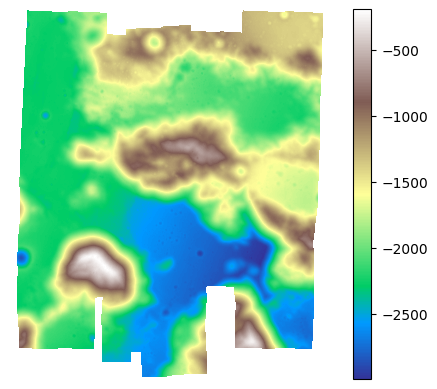
\includegraphics[width=.9\linewidth]{images/apollo_17.png}
\caption{\label{fig:apollo_17}Shaded DEM of Apollo 17 landing site in Taurus-Littrow Valley}
\end{figure}

The slope of a DEM refers to the steepness of terrain at each location in the map (Figure \ref{fig:dem_and_slope}).
Steepness in this context is a measure of the change in elevation over a given distance, often expressed as a percentage or angle in degrees.
Slope is calculated by traversing a 3 x 3 window (Figure \ref{fig:window}) over the DEM\autocite{qiuVoidFillingDigital2019}.
The slope value at the central pixel \emph{e} can be calculated by using the algorithm proposed by Horn \emph{et al.}\autocite{hornHillShadingReflectance1981} :
\begin{align}
Slope &= arctan\sqrt{Slope^2_{we} + Slope^2_{sn}}, \\
Slope_{we} &= \frac{(e_8 + 2e_1 + e_5) - (e_7 + 2e_3 + e_6)}{8 \times Gridsize}, \\
Slope_{sn} &= \frac{(e_7 + 2e_4 + e_8) - (e_6 + 2e_2 + e_5)}{8 \times Gridsize},
\end{align}

\begin{figure}[htbp]
\centering
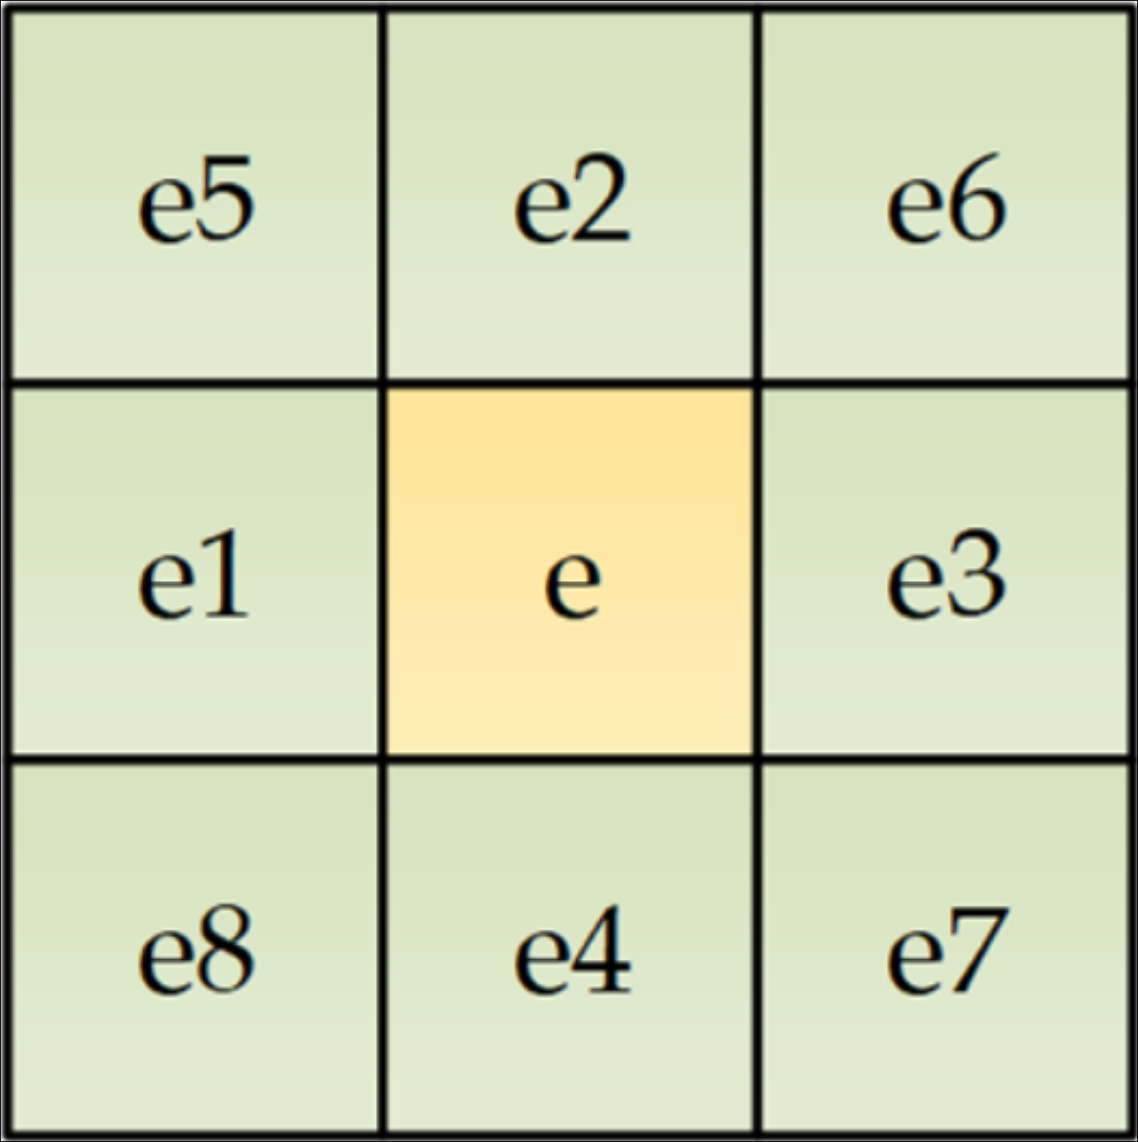
\includegraphics[width=4cm]{images/window.png}
\caption{\label{fig:window}The 3x3 moving window\autocite{qiuVoidFillingDigital2019}}
\end{figure}

\begin{figure}[htbp]
\centering
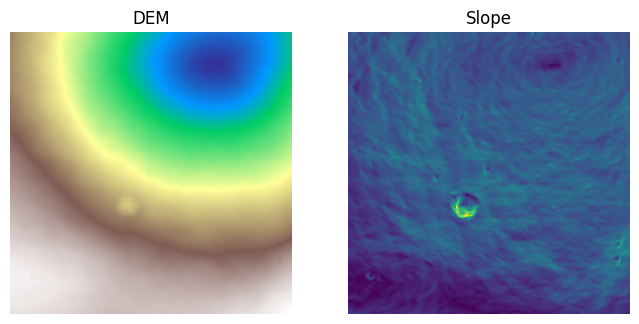
\includegraphics[width=.9\linewidth]{images/dem_and_slope.png}
\caption{\label{fig:dem_and_slope}Section of DEM with computed slope}
\end{figure}

The most common data format for the storage of DEMs is GeoTiff.
A GeoTiff is a type of TIFF (Tagged Image File Format) that with the raw DEM raster data also stores spatial metadata such as pixel resolution (gridsize).
Lunar DEMs are also commonly stored in NASA's PDS (Planetary Data System) archival formats PDS3 and PDS4.
PDS is used to archive multiple kinds of data from planetary science missions, not just DEMs.
Older missions (pre 2011) are typically archived in PDS3, with post 2011 missions using PDS4.
Although stored differently, the raster data in PDS files and GeoTiffs is identical.

The issue of no-data voids is not limited to lunar DEMs, as DEMs are typically constructed using remote sensing technology which is prone to the same errors.

\subsection{Deep Neural Networks}
\label{sec:orgfcdaedb}

Neural networks are a type of machine learning algorithm that is loosely modeled after the structure and function of biological neurons.
An artificial neuron can hold any value, however in most neural networks this value is restricted between 0 and 1 or -1 and 1.
The value a neuron holds is referred to as its activation.
When data is passing forwards through a network, each neuron has an activation determined by the input data.
In a fully connected network, these neurons are arranged into layers, with every neuron in a layer connected to every neuron in the previous layer (Figure \ref{fig:neural_network}).
The first layer is the input layer, the last the output layer and the layers in-between are hidden layers.
In image processing tasks, such as image inpainting, the neurons in the input layer correspond to the pixels of the input image.
The layered structure of the neural network is highly efficient as it allows the network to break down complex problems into smaller steps.

\begin{figure}[htbp]
\centering
\includegraphics[width=.9\linewidth]{images/neural_network.png}
\caption{\label{fig:neural_network}Simple feedforward artifical neural network\autocite{ArtificialNeuralNetwork2023}}
\end{figure}

Each connection between neurons in different layers has an associated weight.
This weight is an indication of how the neuron in the second layer is correlated to the neuron in the first.
A positive weight indicates that when the first neuron has a high activation so should the second, and a negative weight the inverse.
Each neuron also holds a value called a bias, which can be thought of as the minimum weighted sum for the neuron to activate.
To compute the activation of a second layer neuron, take the sum of the activations of the first layer neurons multiplied with their weights and add the bias (Equation \ref{eqn:activation}).
The activation can be any number, however to normalise the signal between a range and add non-linearity to the network the activation is passed through an activation function.
Leaky ReLU (Rectified Linear Unit) (Figure \ref{fig:LeakyReLU}) is an activation function which can introduce sparsity into the network, meaning only a subset of neurons will be activated for any given input, which can reduce the networks complexity and improve its computational efficiency.
The normal ReLU function can can completely deactivate neurons, causing data loss.
For this reason Leaky ReLU was used in the network described by this paper.

\begin{figure}[htbp]
\centering
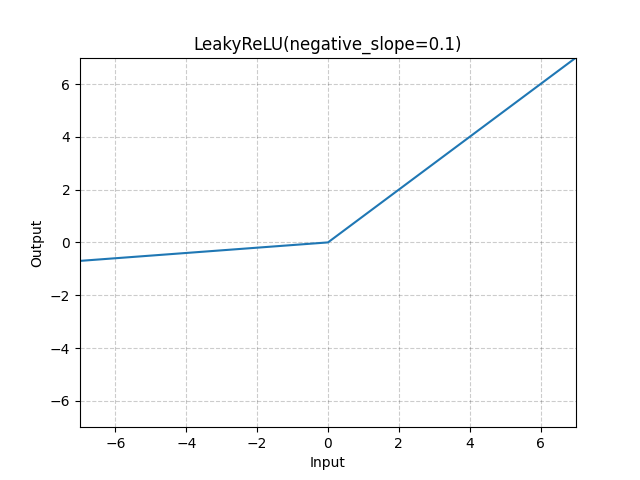
\includegraphics[width=.9\linewidth]{images/LeakyReLU.png}
\caption{\label{fig:LeakyReLU}Leaky ReLU activation function with negative slope of 0.1\autocite{LeakyReLUPyTorchDocumentation}}
\end{figure}

\begin{equation}
\label{eqn:activation}
a^{(1)}_0 = LeakyReLU(w_{0,0}a^{(0)}_0 + w_{0,1}a^{(0)}_1 + \cdots + w_{0,n}a^{(0)}_n + b_0)
\end{equation}

As the equations are linear, to efficiently compute the activation of every neuron in a forward layer, the equations can be stacked into matrices:
\begin{equation}
\begin{bmatrix} a^{(1)}_0 \\ a^{(1)}_1 \\ \vdots \\ a_n^{(1)} \end{bmatrix} = LeakyReLU \left( \begin{bmatrix}w_{0,0} & w_{0,1} & \dots & w_{0,n} \\ w_{1,0} & w_{1,1} & \dots & w_{1,n} \\ \vdots & \vdots & \ddots & \vdots \\ w_{k,0} & w_{k,1} & \dots & w_{k,n} \end{bmatrix} \begin{bmatrix} a_0^{(0)} \\ a_1^{(0)} \\ \vdots \\ a_n^{(0)} \end{bmatrix} + \begin{bmatrix} b_0 \\ b_1 \\ \vdots \\ b_n \end{bmatrix} \right)
\end{equation}

A cost function such as Mean Squared Error (MSE) is used to measure how well the network is performing.
As the network is itself a function, the cost function is a function which takes all the weights and biases of the network as inputs and returns a value describing how well these weights and biases perform.
A neural network is trained with the following steps.
Input data is propagated forwards through the network layer by layer.
The cost function is then evaluated using the predicted output and the actual output, with the error between the two values calculated.
The error is then backpropagated through the network, layer by layer, starting from the output layer.
The desired output of the output layer is known, so by working backwards layer by layer the activations of each neuron that would have resulted in the desired output can be calculated.
The error at each layer is used to calculate the gradient of the cost function with respect to the weights of that layer.
The weights and biases of the network are updated using the gradients calculated during backpropagation by using an optimisation algorithm such as stochastic gradient descent (SGD), which adjusts the weights and biases in a way that takes a step down the gradient towards a local minimum of the cost function; with the steeper the gradient the greater the step taken.
The network can become stuck in a local minimum, as it is impossible to know what the true minimum is, only the downwards direction is known.
An analogy for this would be rolling a ball down a hill.

As calculating the gradient for the entire dataset is very computationally difficult, the data is batched, with the cost function calculated for each example in a batch and then averaged to get a single cost value for the batch - which is then backpropagated.
An epoch is the entire set of training data. It normally takes multiple epochs of training data for the network to converge at a set of weights that minimise the cost function.

A deep neural network is functionally the same, however it involves more hidden layers than the classical network described above.
\subsubsection{Convolutional Neural Networks}
\label{sec:org29b0a43}

\subsubsection{Generative Adversarial Networks}
\label{sec:orgca64abd}

\subsection{Poisson Blending}
\label{sec:org7b2e31a}
Due to the similarity with images, image processing techniques can be applied to the DEMs.
In this paper, the technique of poisson seamless cloning\autocite{perezPoissonImageEditing2003} was used as a post processing step to remove any boundary between the infilled area and original DEM.

\section{Specification}
\label{sec:org4d1300a}

\section{Design}
\label{sec:org41a7939}

\section{Implementation and Testing}
\label{sec:orge2d3233}

\section{Evaluation / Testing}
\label{sec:org8c16e97}

\section{Description of the final product}
\label{sec:org2028791}

\section{Appraisal}
\label{sec:orgd125035}

\section{Summary and Conclusions}
\label{sec:org53a5bf7}

\section{Future Work}
\label{sec:org24fc01a}

\section*{Acknowledgements}

\printbibliography

\section*{Appendices}
\end{document}